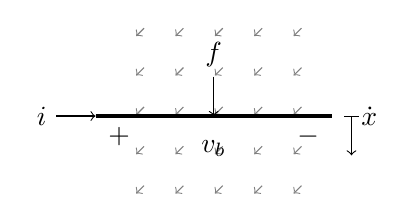
\begin{tikzpicture}[x=1cm,y=1cm,z=-.1cm]
\foreach \x in {0, .5, 1, 1.5, 2}
 \foreach \y in {0, .5, 1, 1.5, 2}
  {
    \draw[->,color=gray] (\x,\y,0) -- (\x,\y,1);
    }
    
 \draw[very thick] (-.5,1,1.15) -- node[pos=.1,below] {$+$} node[pos=.5,below=5pt] {$v_{b}$} node[pos=.9,below] {$-$} (2.5,1,1.15);
 \draw[->] (-1,1,1.15) node[left] {$i$} -- (-.5,1,1.15);
 \draw[->] (1,1.5,1.15) node[above] {$f$} -- (1,1,1.15);
 \draw[|->] (2.75,1,1.15) node[right] {$\dot{x}$} -- ++(0,-0.5,0);
\end{tikzpicture}